\section{Productivity Focused Platforms} \label{chapter3:software-productivity}

\cit{It is becoming increasingly important to the data-processing industry to be able to produce
[programming systems] % more programming systems and produce them with fewer errors,
at a faster rate, and in a way that modifications can be accomplished easily and quickly.}{W. Stevens, G. Myers, L. Constantine \cite{Stevens1974}.}

In order to improve and maintain a software system, it is important to holds in mind a mental representation of its implementation.
As the system grows in size, the mental representation becomes more and more difficult to grasp.
Therefore, it is crucial to decompose the system into smaller subsystem easier to grasp individually.
% This section presents academic propositions for software productivity, and then presents how the industry adapted these solutions to meet their needs.
% Finally, this section presents the limitations of the presented solutions.

% \nt{Interesting, but to be rewritten: 
% Architects, and mechanical engineers draw codified plans to share their mental representations with peers and building teams.
% software design is an exception in that the implementation is both the shared mental representation, and the actual product.
% The mental representation is often lost in technical details and optimizations for the actual product.
% }

\cit{Measuring programming progress by lines of code is like measuring aircraft building progress by weight.}{Bill Gates}

Section \ref{chapter3:software-productivity:modularity} presents the modular programming paradigms, and their programming models, oriented toward productivity.
Section \ref{chapter3:software-productivity:adoption} presents the adoption of the implementations of modular programming languages.
Section \ref{chapter3:software-productivity:performance-limitations} presents the consequences of the modularity on performance.
Finally, section \ref{chapter3:software-productivity:summary} summarizes the three previous sections in a table.

\subsection{Modular Programming} \label{chapter3:software-productivity:modularity}

\begin{figure}[!h]
\begin{center}
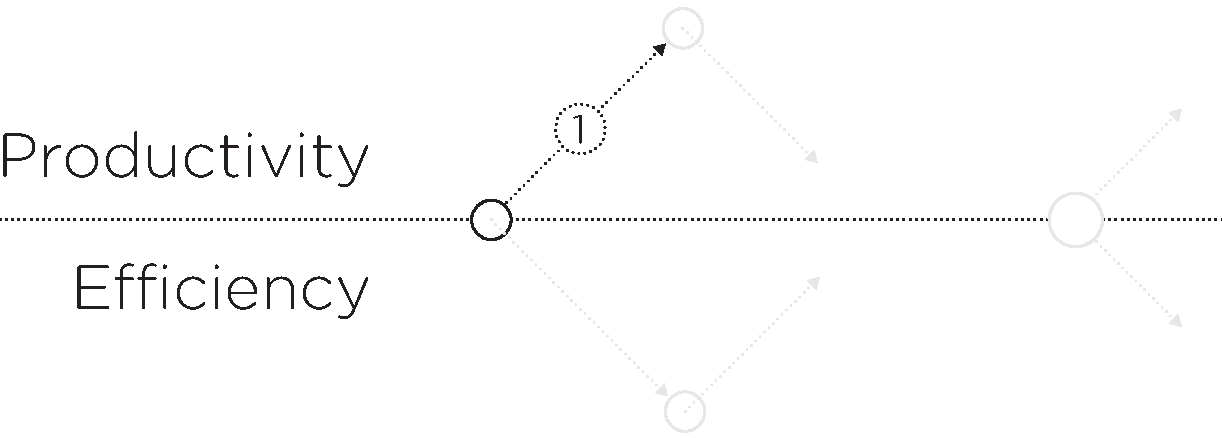
\includegraphics[width=0.6\textwidth]{../resources/state-of-the-art-1.pdf}
\end{center}
\caption{Focus on Productivity}
\label{fig:state-of-the-art-1}
\end{figure}

% The modularity of a software implementation is about enclosing subproblems and composing them through relevant interface abstractions.
% % It allows greater design to emerge from the composition of smaller components.
% It improves the productivity of an implementation, as illustrated in figure \ref{fig:modular-programming-state-of-the-art}.
% It allows to limit the understanding required to contribute to a module \cite{Stevens1974}.
% And it reduces development time by allowing several developers to simultaneously implement different modules \cite{Wong2009,Cataldo2006}.

% % \nt{Read and include \cite{Simon1962}}

% % \subsubsection{Design Choices} \label{chapter3:software-productivity:design-choices}

% % \nt{TODO this introduction is not very clear}
% % In the decomposition of a large problem into smaller subproblem, there is two design choices.
% % The first one is the granularity, and organization of the subproblems within the system decomposition.
% % The second one is the organization of the implementation within the subproblems to improve productivity.

% % \nt{reduce all these paragraph into a concise one and move it into the introduction}

% % \paragraph{System Decomposition}

% \illustration{spaghetti programming}
% Modular Programming stands upon Structured Programming \cite{Dijkstra1970}.
% % Dijkstra firstly developed the concept of Structured Programming \cite{Dijkstra1970}, which later led to modular programming.
% % It is defined as \textit{the systematic use of abstraction to control a mass of details, and also a means of documentation which aids program design} \cite{Knuth1974}.
% It draws clear interfaces around a piece of implementation so that the execution is enclosed inside.
% At a fine level, it helps avoid spaghetti code \cite{Dijkstra1968a}, and at a coarser level, it structures the implementation \cite{Dijkstra1968} into modules, or layers.
% % The next paragraph explains further the criteria to draw the borders around modules.
% \illustration{lasagna programming}
% Encapsulate a specific design choice in each module, so that it is responsible for one and only one concern, isolate its evolution from impacting the rest of the implementation \cite{Parnas1972, Tarr1999, Hursch1995}.
% Examples of such separation of concerns are the separation of the form and the content in HTML / CSS, or the OSI model for the network stack.

% The criteria to define modules to improve productivity are coupling and cohesion \cite{Stevens1974}.
% The coupling defines the strength of the interdependence between modules, while cohesion defines how strongly the features inside a module are related.
% Low coupling between modules and high cohesion inside modules helps logically organize, and understand the implementation.
% Hence, it improve its productivity.

% The composition of modules with low coupling is provided by encapsulation, higher-order programming and lazy evaluation.
% Hence, the criteria to analyze the solutions presented in this section regarding productivity are :
% \begin{itemize}
% \item encapsulation mechanism
% \item presence of higher-order programming
% \item presence of lazy evaluation, or stream composition
% \end{itemize}
% The last two criteria provide composition abstractions to design solutions from smaller components.
% Encapsulation and composition are the features in modular programming that produce productivity.

% The next paragraphs present the last two criteria \ref{chapter3:software-productivity:modularity:features}, and  then the main programming models, section \ref{chapter3:software-productivity:modularity:programming-models}.

% \paragraph{Decomposition Criteria}

% \nt{move this paragraph closer to OOP ?}
% The criteria to define modules to improve productivity are coupling and cohesion \cite{Stevens1974}.
% The coupling defines the strength of the interdependence between modules, while cohesion defines how strongly the features inside a module are related.
% Low coupling between modules and high cohesion inside modules helps logically organize, and understand the implementation.
% Hence, it improve its productivity.
% The next paragraph presents the approach to build modules helping with the evolution of the implementation.

% \paragraph{Development Evolution}

% \nt{productivity also relies on supporting implementation evolution}

% The modular organization should isolate the evolution of a module from impacting the rest of the implementation.
% Encapsulate a specific design choice in each module, so that it is responsible for one and only one concern, isolate its evolution from impacting the rest of the implementation \cite{Parnas1972, Tarr1999, Hursch1995}.
% Examples of separation of concerns are the separation of the form and the content in HTML / CSS, or the OSI model for the network stack.
% The information hiding principle advocates to encapsulate a specific design choice in each module.
% The Separation of Concerns advocates each module to be responsible for one and only one specific concern.

% Figure \ref{fig:modular-programming-state-of-the-art} illustrates an overview of the direction of modular programming regarding the general trends in software design.
% Section \ref{chapter3:software-productivity:design-choices} presents the decomposition.

% \subsubsection{Programming Models} \label{chapter3:software-productivity:programming-models}

% \subsubsection{Features} \label{chapter3:software-productivity:modularity:features}

% \paragraph{Higher-Order Programming}
% \nt{If possible, include this reference : Continuations and coroutines \cite{Haynes1984}}

% Higher-order programming allows to manipulate functions like any other primary value : to store them in variables, or to pass them as arguments.
% It replaces the need for most modern object oriented programming design patterns \ftnt{http://stackoverflow.com/a/5797892/933670} with Inversion of Control \cite{Johnson}, the Hollywood Principle \cite{Sweet1985}, and Monads \cite{Wadler1992}.
% Higher-order programming help loosen coupling, thus improve productivity.

% In languages allowing mutable state, higher-order functions are implemented as closure, to preserve the lexical scope \cite{Sussman1998}.
% A closure is the association of a function and a reference to the lexical context from its creation.
% It allows this function to access variable from this context, even when invoked outside the scope of this context.
% \nt{next sentence is redundant with the suit}
% It eventually tangles the memory references so that it requires a global memory.

% \paragraph{Lazy Evaluation}

% Lazy evaluation is an evaluation strategy allowing to defer the execution of a function only when its result is needed.
% % And according to \cite{Hughes1989}, \textit{Abelson and Sussman stress that streams (lazy list) is a powerful tool for structuring programs \cite{Sussman1983}.
% The lazy evaluation of lists is equivalent to a stream with a null-sized buffer, while the opposite, eager evaluation, corresponds to an infinite buffer \cite{VanRoy2003}.
% \nt{find another transition}Indeed, the dataflow programming paradigm resulting from lazy lists is particularly adapted for stream processing applications.

% \nt{This paragraph is not very clear}
% The lazy evaluation, as well as streams are powerful tools for structuring modular programs \cite{Sussman1983}.
% Lazy evaluation allows the execution to be organized as a concurrent pipeline, as the stages are executed independently for each element of the stream.
% But this concurrency requires immutability of state, or at least isolation of side-effects.\nt{why ? explain or point to the explanation}
% The next section addresses the consequences of higher-order programming and lazy evaluation on parallelism.


% \subsubsection{Programming Models} \label{chapter3:software-productivity:modularity:programming-models}

The next paragraphs presents the different programming model regarding their support to modular programming and productivity.
% They represent the number \circled{1} in figure \ref{fig:modular-programming-state-of-the-art}.

\subsubsection{Imperative Programming}

Imperative programming is the very first programming paradigm, as it evolves directly from the hardware architectures.
It allows to express the suite of operation to carry sequentially on the computing processor.
% Lots of programming languages feature imperative programming.
Most imperative languages provide encapsulation with modules but not higher-order programming, nor lazy evaluation.
The implementations of Imperative Programming 

\subsubsection{Object Oriented Programming}

\illustration{multiple cells communicating}

% Alan Kay, who coined the term, states that Object Oriented Programming (OOP) is about message-passing, encapsulation and late binding.
% (There is no academic reference for that, only a public mail exchange\ftnt{http://userpage.fu-berlin.de/~ram/pub/pub\_jf47ht81Ht/doc\_kay\_oop\_en}.)
% Message-passing and late binding loosen coupling between objects, while encapsulation is intended to increase cohesion \ftnt{http://williamdurand.fr/2013/06/03/object-calisthenics/}.
% % Reducing coupling and increasing cohesion are further sought by object calisthenics, in the chapter 6 of \textit{The Thoughtworks Anthology} \cite{Bay2008}

The very first Object-Oriented Programming (OOP) language was Smalltalk \cite{Goldberg1984}.
It defined the core concepts as message passing and encapsulation %, and dynamic binding
\ftnt{http://userpage.fu-berlin.de/~ram/pub/pub\_jf47ht81Ht/doc\_kay\_oop\_en}.
Nowadays, the emblematic figures in the software industry are C++ \ImplementationsOf{Object-Oriented Programming}.
% Though, the trend seems to digress from these languages to evolve toward a more dynamic approach.
% Indeed Javascript adopts some functional features such as dynamic typing and higher-order functions \cite{Ecma1999}.}
They provide encapsulation with Classes, and allows passing mutable structures for performance reasons.
They recently introduced higher-order programming with lambda expressions.

\subsubsection{Functional Programming} \label{chapter3:software-productivity:programming-models:functional-programming}

% \cit{All problems in computer science can be solved by another level of indirection}{Butler Lampson}

The definition of pure Functional Programming resides in manipulating only expressions and forbidding state mutability, replaced by message passing.
The absence of state mutability makes a function side-effect free, hence their execution can be scheduled in parallel.
But it implies heavy message passing, which negatively impact performances.
The most important pure Functional Programming languages are \ImplementationsOf{Functional Programming}.
They provide encapsulation, higher-order programming and lazy evaluation.

\subsubsection{Multi-Paradigm}

The functional programming concepts are also implemented in other languages along with mutable states and object-oriented concepts.
% The two main references of Object-Oriented Programming, Java and C++, adopted higher-order functions in their last version, Java 8 and C++11.
Major recent programming languages, including Java 8 and C++ 11, now commonly present \textbf{higher-order functions} and \textbf{lazy evaluation}. % to help loosen the couple between modules. %, define more generic and reusable modules.
% Moreover, they provide reflective programming, and other meta-programming techniques.
\textit{In fine}, it helps developers to write applications that are more maintainable, and favorable to evolution \cite{Hughes1989,Turner1981}.
These recent multi-paradigms languages such as \ImplementationsOf{Multi Paradigm} combine the different paradigms to help developer building applications faster.
% They provide encapsulation, higher-order programming and stream composition.

\paragraph{}

Table \ref{tab:productivity-modularity} presents a summary of the analysis of the programming models presented in the previous paragraphs.

\ModularProductivityTable{tab:productivity-modularity}

% \begin{table}[h!]
% \small
% \begin{tabu} to \linewidth {@{} l X[l] c c c c @{}}
% %
% % \multicolumn{3}{c}{}  & \lab{Concurrency} & \multicolumn{2}{|c}{Parallelism} \\
% Model & Implementations    & \lab{Composition} & \lab{Encapsulation} & $\to$ & \lab{Productivity} \\
% \tabucline[.5pt]{-}%
% Imperative Programming         & C                                             & \X & \V && \X \\ \tabucline[on .5pt]{-}
% Object-Oriented Programming    & C++, Java                                     & \V & \V && \V \\ \tabucline[on .5pt]{-}
% Functional Programming         & Scheme, Miranda, Haskell                      & \V & \V && \V \\ \tabucline[on .5pt]{-}
% Multi Paradigm                 & Javacript, Python, Ruby, Go                   & \V & \V && \V \\
% \tabucline[.5pt]{-}
% \end{tabu}
% \caption{Analysis of the state of the art in modular programming regarding productivity}
% \label{tab:productivity-modularity}
% \end{table}

\subsection{Adoption} \label{chapter3:software-productivity:adoption}

\begin{figure}[!h]
\begin{center}
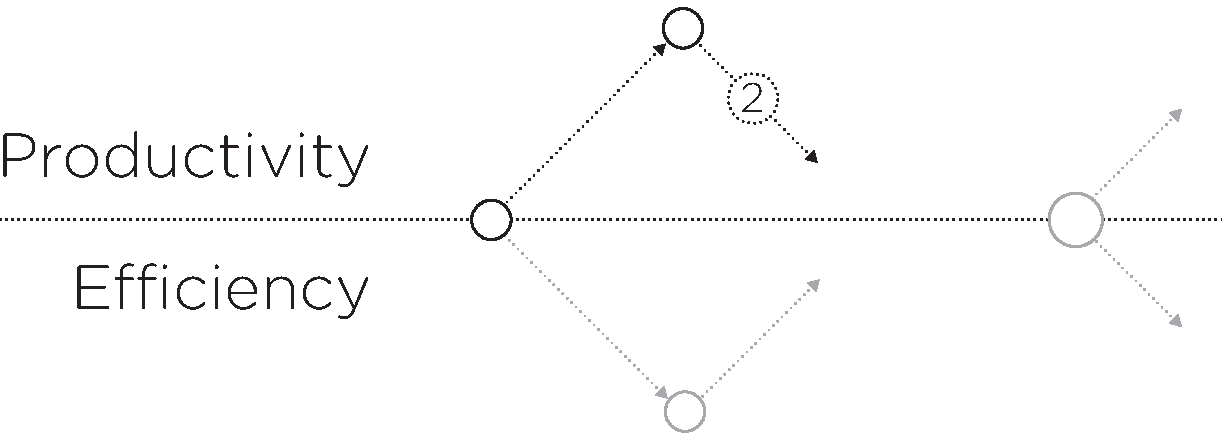
\includegraphics[width=0.6\textwidth]{../resources/state-of-the-art-2.pdf}
\end{center}
\caption{Steering back toward Performence Efficiency}
\label{fig:state-of-the-art-2}
\end{figure}

% A system is maintainable only if there is people willing to maintain it.
% For people to widely adopt a programming language, it needs to be features a balance between performance and productivity.
% It forces the modular programming models to be implemented taking into account not only productivity, but performance as well.
% The balance is steered back toward performance, as illustrated in figure \ref{fig:state-of-the-art-2}.

% Indeed, the immutability of pure functional programming impact performance too negatively to be wildly used in industrial context.
% And the pure object-oriented programming lacks composition abstractions, like higher-order programming and lazy evaluation.
% As a result, the multi-paradigm scripts tends to be better compromises between modularity and performance.
% And the data of this section proves it.

% The criteria to analyze the solutions presented in this section regarding the adoption are the adoption in :
% \begin{itemize}
% \item the community,
% \item the industry,
% \item web technologies
% \end{itemize}
% The first two criteria make sure that the technology is growing organically with a passionate community, and backed by industrial needs.
% The last criteria assures the fitting of the technologies with our economical context of a web application.
The next paragraphs presents the adoption of Javascript, and the other implementations of the presented programming model.
% ->_>_>_>_> These implementations steer back from productivity into performance efficiency, as shown by \circled{2} in figure \ref{fig:modular-programming-state-of-the-art-2}.

% The rise of Javascript is indisputable on the web, and seems to be rising in the software industry as well.
% But it is difficult to give an accurate representation of the situation because the software industry often maintains a fog of war to try to keep an edge.
% The following paragraphs report some efforts to clear up the situation.
% More detailed informations are available section \ref{appendix:langpop}.

\subsubsection{Community}

\paragraph{Available Resources}

As of December 2015, Javascript ranks 8th according to the TIOBE Programming Community index, and was the most rising language in 2014.
This index measure the popularity of a programming language with the number of results on many search engines.
% However, this measure is controversial as the number of pages doesn't represent the number of readers.
And it ranks 7th on the PYPL.
The PYPL index is based on Google trends to measure the number of requests on a programming language.
% However, it is limited to Google searches.

From these indexes, the major programming languages are Java, C++, C, C\# and Python.
% The preponderance of Object-Oriented Languages in these results is explained by the lag of these indexes.
% Java and C/C++ were very popular and helped bring the explosion of the web.
These languages are still widely used by their communities and in the industry.
% Though, the next paragraphs bring a more actual vision.

\nt{TODO graphical ranking of TIOBE and PYPL}

\paragraph{Developers Collaboration Platforms}

Online collaboration tools give an indicator of the number of developers and projects using certain languages.
Javascript is the most used language on \textit{Github}\ftnt{the most important collaborative development platform gathering about 9 millions users.} and the most cited language on \textit{StackOverflow}\ftnt{the most important Q\&A platform for developers.}.
It represents more than \num{320000} repositories on \textit{Github}.
The second language is Java with more than \num{220000} repositories.
It is cited in more than \num{960000} questions on \textit{StackOverflow} while the second is Java with around \num{940000} questions.
% According to \textit{Black Duck Software}\ftnt{https://www.blackducksoftware.com/} it is the second language used in open source projects.
% C is first, C++ third and Java fourth.\ftnt{https://www.blackducksoftware.com/resources/data}
% These four languages represent about 80\% of all programming language usage in open source communities.
And according to a survey by \textit{StackOverflow}, it is currently the language the most popular\ftnt{http://stackoverflow.com/research/developer-survey-2015}.
Moreover, the Javascript package manager, \textit{npm}, has the most important and impressive package repository growth.

\nt{TODO include so survey graph}

\nt{TODO redo this graph, it is ugly.}
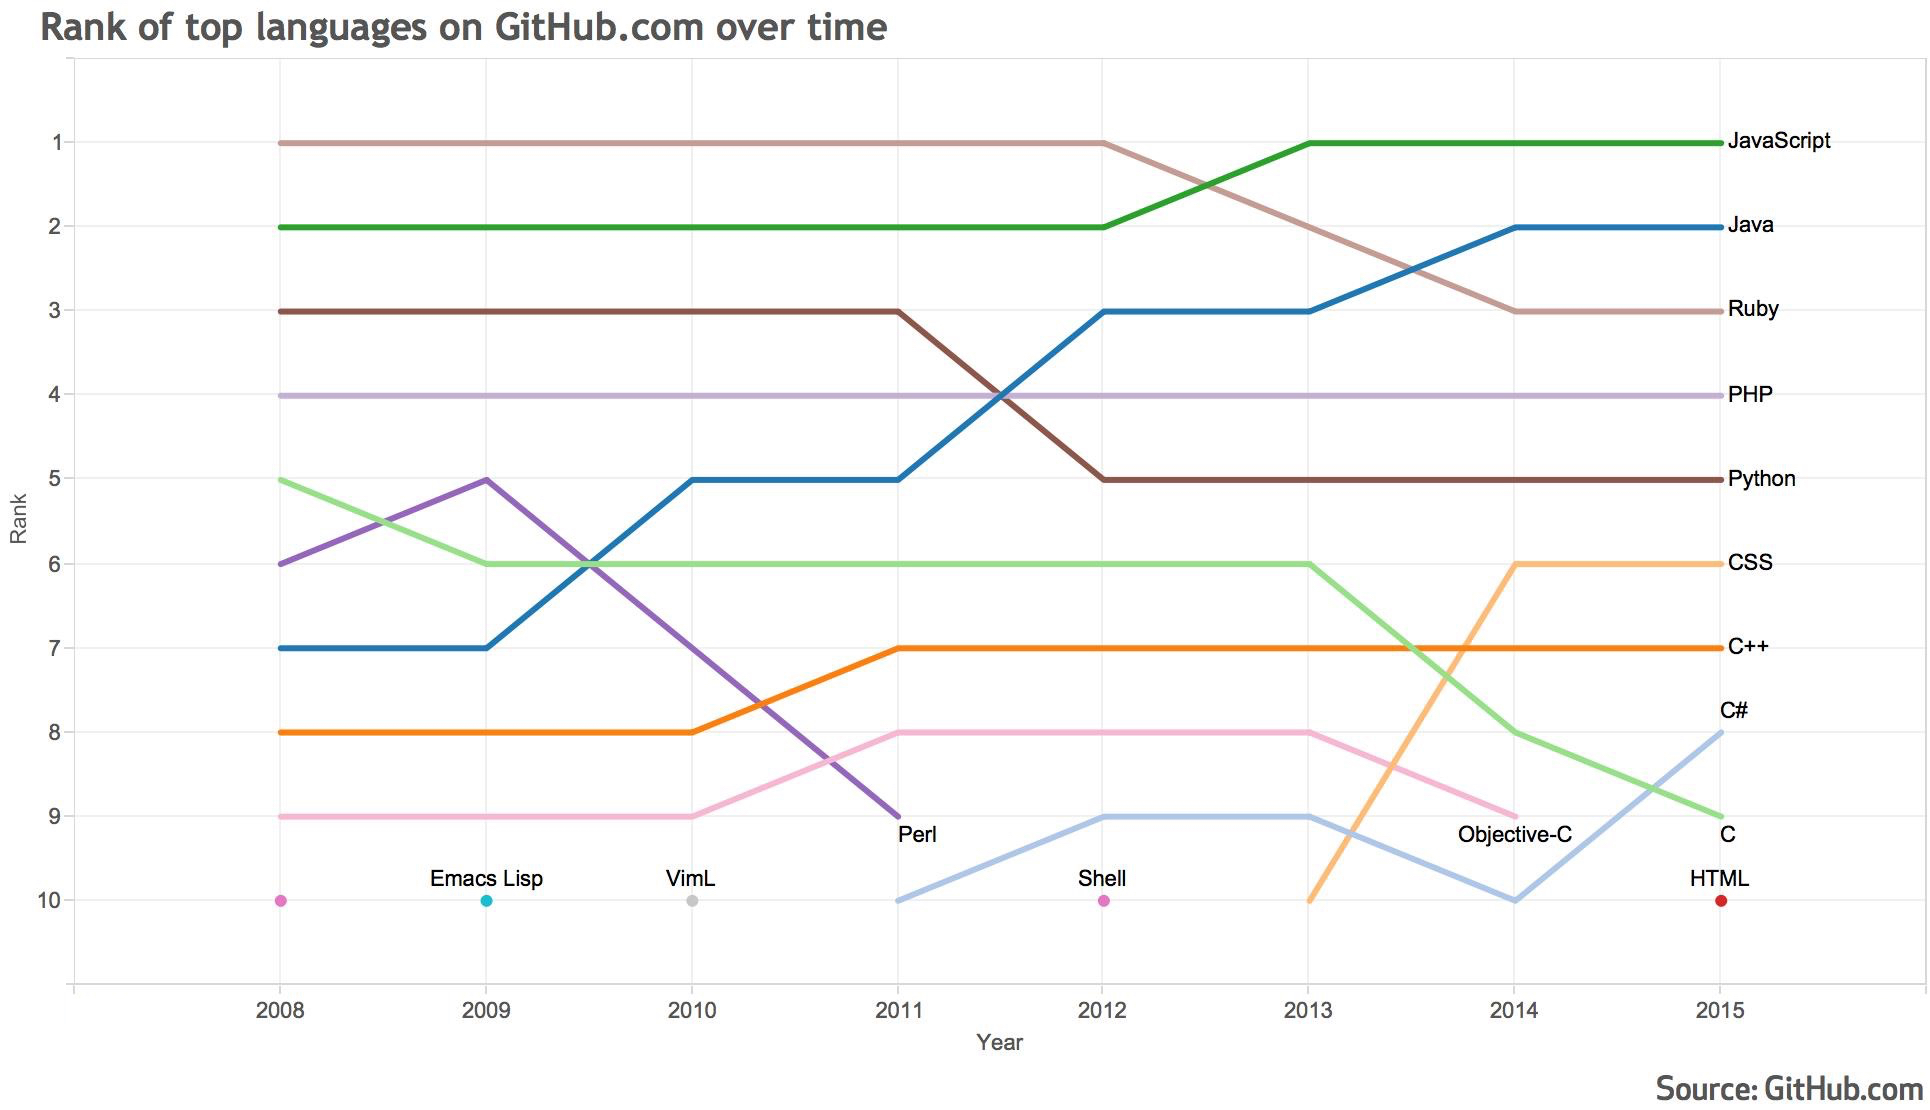
\includegraphics[width=0.9\linewidth]{../../data/js-trends/github-ranks}\ftnt{https://github.com/blog/2047-language-trends-on-github}

\nt{TODO graphical ranking of the tags in StackOverflow}

% \nt{TODO redo this graph, it is ugly.}
% 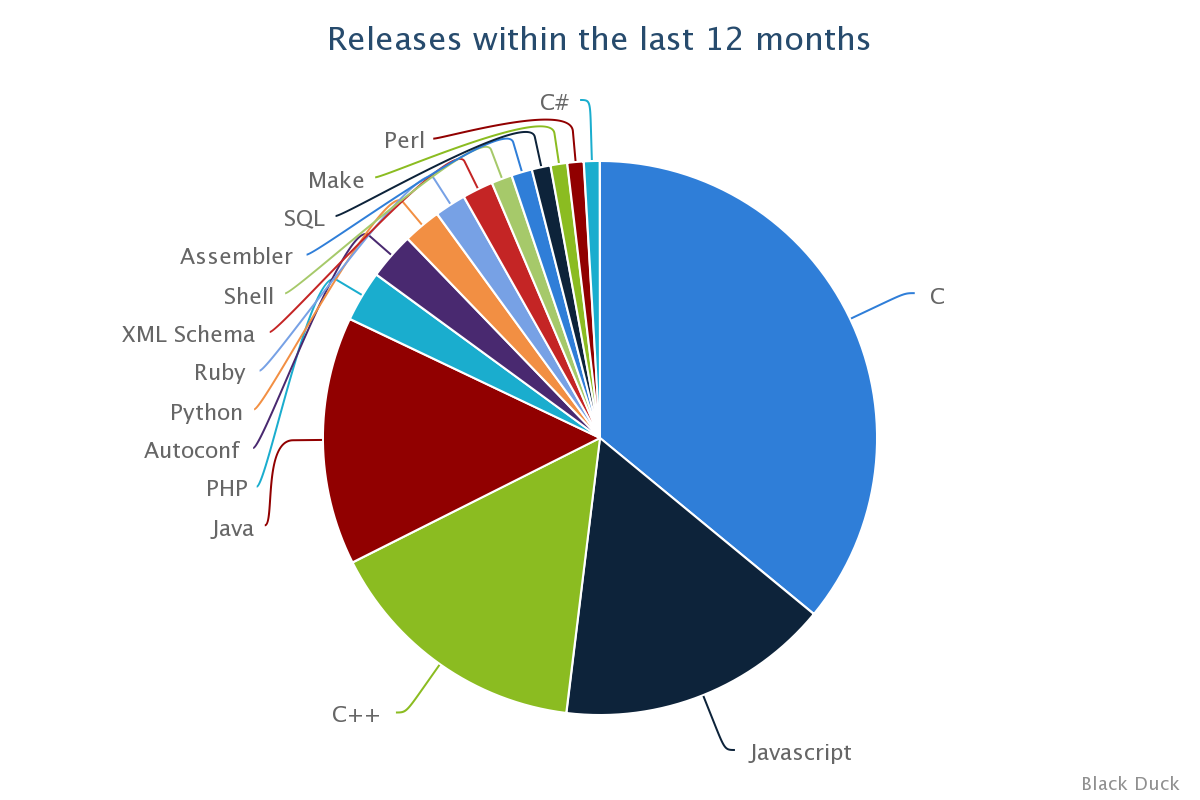
\includegraphics[width=0.9\linewidth]{../../data/js-trends/black-duck-15}

\nt{TODO redo this graph, it is ugly.}
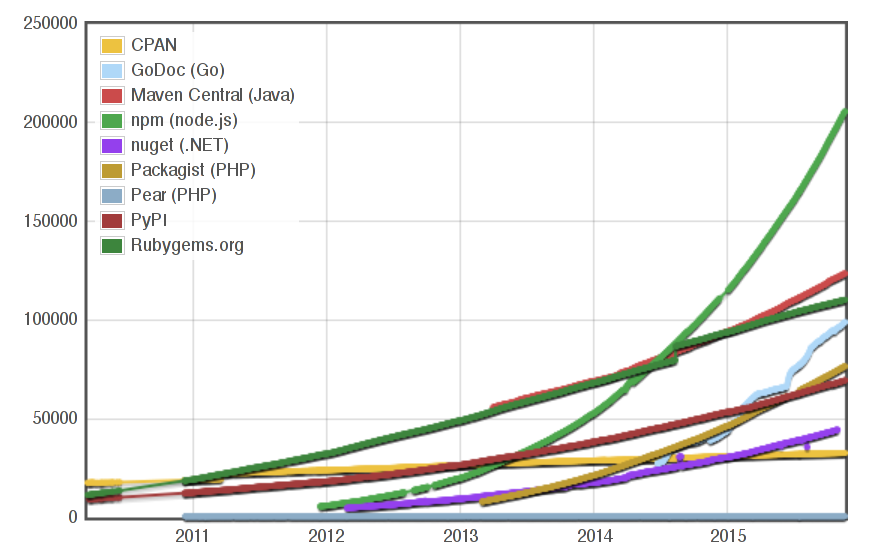
\includegraphics[width=0.9\linewidth]{../../data/js-trends/modulecounts}

\subsubsection{Industry}

The actors of the software industry tends to hide their activities trying to keep an edge on the competition.
The previous metrics represent the visible activity but are barely representative of the software industry.
The trends on job opportunities give some additional hints on the situation.
Javascript is the third most wanted skill, according to \textit{Indeed}\ftnt{http://www.indeed.com}, right after SQL and Java.\ftnt{http://www.indeed.com/jobtrends?q=Javascript\%2C+SQL\%2C+Java\%2C+C\%2B\%2B\%2C+C\%2FC\%2B\%2B\%2C+C\%23\%2C+Python\%2C+PHP\%2C+Ruby\&l=}
Moreover, according to \textit{breaz.io}\ftnt{https://breaz.io/}, Javascript developers get more opportunities than any other developers.
Javascript is increasingly adopted in the software industry.

\nt{TODO redo this graph, it is ugly.}
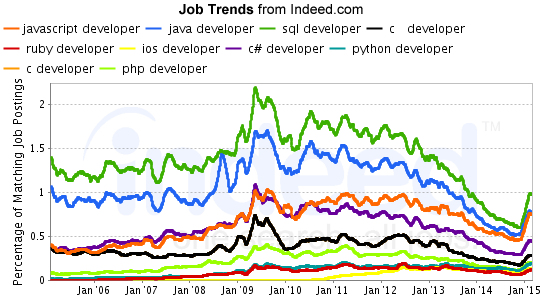
\includegraphics[width=0.9\linewidth]{../../data/js-trends/jobgraph}

\paragraph{}

Table \ref{tab:productivity-adoption} presents a summary of the analysis of the programming models presented in the previous paragraphs.

\ModularAdoptionTable{tab:productivity-adoption}

\subsection{Efficiency Limitations} \label{chapter3:software-productivity:efficiency-limitations}

Eventually, the presented languages are hitting a wall on their way to performance.

All the languages presented previously provide global memory abstraction on which to rely to assure encapsulation and composition -- either mutable state or immutable state.
Functional programming relies on immutable message-passing.
It might impacts performance at a fine-grain level because of heavy memory usage.
On the other hand, the synchronization required by mutable state is often hard to develop with \cite{Adya2002}, or avoid parallelism \cite{Pai1999,Krohn2007}.

The only solution to provide performance efficiency is to combine mutable state at a fine-grain level, with synchronization, and immutable state at a coarse-grain level, with message-passing.

% The next paragraph briefly presents the encountered incompatibility between modularity and performance to introduce the next section of this chapter.


% Parallelizing the execution increases the performances \cite{Amdahl1967,Gunther1993}
% But it is limited because accesses to sharing state need to be scheduled sequentially.
% Hence, to increase the parallelism and performance, the concurrent executions need to be independent, or to coordinate to be scheduled sequentially \cite{Gustafson1988,Gunther1996,Nelson1996,Gunther2002}.
% On the other hand, completely forbidding shared state, with immutable state, increase the need for communication because of the additional required synchronization.
% Eventually, the communications induce a greater overhead than the performance increases from parallelization, and it finally negatively impacts the performances.

% To be scalable, a solution needs to allow shared state at a fine grain, where lots of synchronization is required, and where communication would induce a greater overhead than parallelization could compensate. 
% And immutability at a coarse grain, where lesser synchronization is required, and parallelization can be advantageously used.

% Encapsulation aims not to provide this decomposition between sharing and immutable space required for performance scalability.
% It aims to draw a clear boundary around the concern of a module to help understanding it.
% To allow higher-order programming and mutable state, despite encapsulation, languages implement closures, and intermingle the memory between modules.
% It reinforces the need for synchronization and sequentiality.
% 
% Finally, the requirement to enforce the decomposition required for performance scalability are :
% \begin{itemize}
% \item shared state : fine level sequentiality
% \item immutable state : coarse level message passing
% \end{itemize}


The table \ref{tab:productivity-performance} presents the performance limitations of the languages presented in this section.
% It only presents programming languages.
The platforms extending these languages with concurrent or parallel features to provide performances are addressed in the next section.


\ModularEfficiencyTable{tab:productivity-performance}

\subsection{Summary} \label{chapter3:software-productivity:summary}

Table \ref{tab:productivity-synthesis} summarizes the characteristics of the solutions presented in this section.

\ModularSummaryTable{tab:productivity-synthesis}

\endinput






































\nt{read and include 
Octave and python: higher-level scripting languages productivity and performance evaluation, by Chaves, Nehrbass, Guilfoos, Gardiner.
Haskell vs Ada vs C++ vs Awk vs ... an experiment in software productivity, technical report by Hudak and Jones.
An empirical comparison of seven programming languages, by Prechelt.
}

% Pipeline parallelism is relevant for multi-pass algorithms \cite{Conway1963}, and it is particularly efficient for stream processing applications.

% \subsubsection{Efficiency Limitations} \label{chapter3:software-maintainability:limitations}


% Functional programming -> immutability is bad for performance at a fine grain because it implies lots of communication aka memory copy.
% Object Oriented Programming -> for the same reason, oop is not implemented in practice with message passing as the next section will present, even if the initial definition is about message passing.
% IMPORTANT -> immutability is bad for performance at a fine grain.


% Functional programming greatly support modularity to improve the maintainability of an application, and its resilience to evolution.
% However, the closures introduced by higher-order programming require to share the execution context among modules.
% The previous chapter show that sharing makes parallelism difficult.
% It is the reason why that maintainability and performance seem hardly compatible.
% This section explores in further details the limitation of modular programming regarding performances.

% \paragraph{Tighten Memory}

% Closures are implemented in languages using a global memory.
% And by exchanging closures, two modules intricately share their contexts of execution.
% Higher-order programming loosen the couple on the implementation level of the modules, but tighten it on the execution level.
% It improves modularity, but it inherently worsens the parallelization hence the performance scalability.

% \paragraph{Scalability Limitations}

% Parallelizing the execution increases the performances \cite{Amdahl1967,Gunther1993}
% But the parallelism is limited because the execution portions sharing state need to be scheduled sequentially.
% Hence, to increase the parallelism and performance, the concurrent executions need to be independent, or to coordinate to be scheduled sequentially \cite{Gustafson1988,Gunther1996,Nelson1996,Gunther2002}.
% We explain further the reasons of these limitations, and the improvement solutions in the next section.

% \nt{move this citation elsewhere}
% \cit{No matter how great the talent or efforts, some things just take time. You can't produce a baby in one month by getting nine women pregnant.}
% {Warren Buffett\ftnt{http://www.goodreads.com/quotes/476827-no-matter-how-great-the-talent-or-efforts-some-things}}


% \paragraph{}






\nt{TODO the transition is not very clear}
The modular organization of implementation is opposed to the organization favoring the parallelization of the execution.
The former organization supports the development scalability, while the latter supports performance scalability.
A program cannot trivially follow an organization that support both development evolution, and performance.
\nt{explain more clearly why}

The next section shows the improvements for performance and parallelism .
Then, section \ref{chapter3:software-performance} shows the techniques for parallelism.

\subsection{Efficiency Improvements} \label{chapter3:software-maintainability:performance}

INDUSTRY INDUSTRY INDUSTRY

To assure its integrity, the global state of an application imposes the concurrent executions to coordinate their accesses to be atomic and exclusive\nt{explain these terms}.
This coordination is responsible of the atomicity, and exclusivity of the accesses.
\nt{the next two sentences are not clear}
It assures the invariance of the state during its atomic manipulation.
So that developers can group operations in atomic manipulations so as to avoid corruption of the state.

The invariance is assured differently depending on how the state is shared among the concurrent execution.
To increase performance, concurrent executions needs to be as independent as possible to be executed in parallel \ftnt{http://joeduffyblog.com/2010/07/11/thoughts-on-immutability-and-concurrency/}.
% Isolation is independent processes
% Immutability Immutability
% Synchronization is event-loop, multi-thread, lock-free
\begin{description}
  \item[Isolation] If different concurrent executions are commutative \cite{Rinard1996,Clements2013a}, and they share no portion of the state then they can be isolated and executed in parallel.
  \item[immutable state] Otherwise, the sharing state portions needs to be immutable to conserve invariance and parallel execution \cite{Gordon2012,Matsakis2012a}.
  \item[shared state] If different concurrent executions needs mutation on the state, their accesses are scheduled sequentially.
\end{description}

\begin{center}
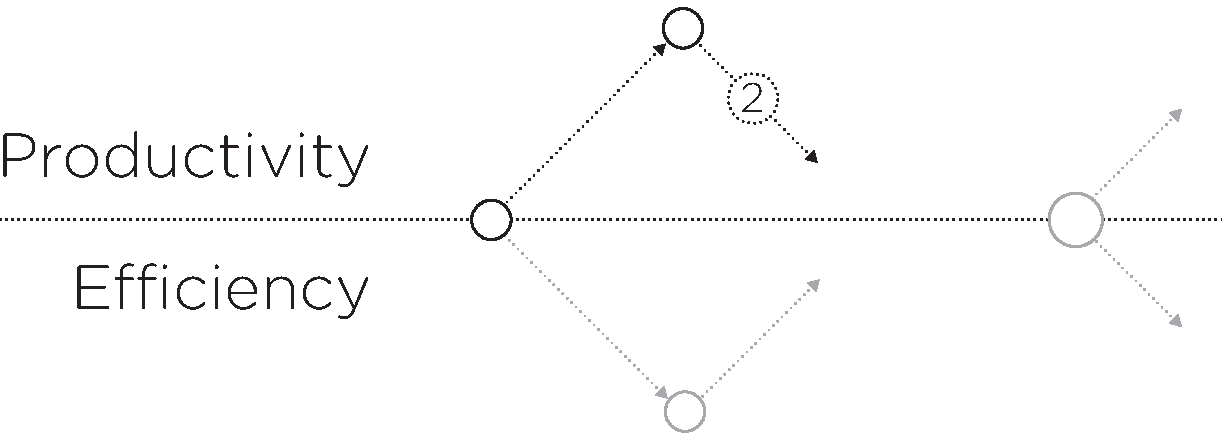
\includegraphics[width=0.6\textwidth]{../resources/state-of-the-art-2.pdf}
\end{center}

The next few paragraphs present the different models to assure invariance in concurrent execution, while conserving modular programming, \comment{as illustrated in the schema above}.
Section \ref{chapter3:software-maintainability:performance:concurrent-programming} presents the programming models providing synchronization and immutability for concurrent executions.
Section \ref{chapter3:software-maintainability:performance:compilation} presents compilation methods to parallelize sequential programs.

% Dynamic Isolation + Making asynchronous parallelism safe for the world \cite{Jr1990}


\subsubsection{Adaptation of the theoretical models to the industry}

The major program for modular programming is C, but it evolved with OOP into C++.
Nowadays, the major emblematic figures of OOP in the software industry are C++ and Java \cite{Gosling2000,Stroustrup1986}.
All these languages are far from the theoretical models proposed by the academy.
They get back to a more imperative model for performance reason.

Though, the trend seems to digress from these languages to evolve toward a more dynamic approach, closer to Functional Programming.
Functional programming like Haskell are not very efficient.
The major argument is that they are hell of a lot more expressive, but eventually, the lack of state is confusing and inefficient, and few developers adopt them.
Exactly like oop, or the actor model, immutability at a fine granularity is inefficient.
The good granularity is synchronization at a fine granularity (within functions), immutability and isolation at a coarse granularity (between modules).

Indeed Javascript adopts some functional features such as dynamic typing and higher-order functions \cite{Ecma1999}, because they are expressive, but conserve the state mutability for its performance.

The precedent chapter present the adoption of different languages, and particularly of Javascript.
No language from the academy is broadly adopted.
But more general / balanced / multi-paradigm languages are widely adopted (C/C++, Java, Javascript, Python etc ...).



% It is easy to understand the parallelism in a cooking recipe because the interdependencies between operations are trivial.
% It seems obvious that melting chocolate is independent from whipping up egg whites.
% % Because chocolate and egg whites are different ingredients.
% This distinction between chocolate and egg whites is trivial.
% % ... comes from the modifications to the state.
% While the distinctions within the state of an application are more intricate.
% This makes concurrent application more difficult to design and implement.


% \paragraph{Transition on parallel programming}

% The definition of separation of concerns given in this section is orthogonal to the original meaning coined by Dijkstra .
% It is interesting to note this difference, as it is related directly to this thesis.
% % Initially, it meant the ability to reason independently about different concern about a software system.
% The initial definition was about analyzing independently how a system meets different concerns.
% Dijkstra gives the example of analyzing independently correctness and efficiency.
% It is impossible to encapsulate correctness, or efficiency in a module, they concern the whole system.
% In this respect, this thesis is oriented towards dissociating the concern of development evolution and of performance.
% That is to be able to reason on the maintainability of a program, independently than of its performance, and vice versa.
% % This seems challenging as D. Parnas opposed these two concerns.
% It is the challenge presented by D. Parnas when he opposed the two concerns in \cite{Parnas1972}.

% This thesis investigates further this opposition to dissociate the concern of evolution and the concern of performance in the case of a web application.
% The next section investigates the first concern, and presents the major programming models used to improve the evolution of an application.

\endinput



remote first Zack Holman : promote asynchronous communication
\ftnt{http://zachholman.com/posts/remote-first/}
+
Conway's law
\cit{Organizations which design systems [...] are constrained to produce designs which are copies of the communication structures of these organizations.}
{M. Conway \cite{Conway1968}}



\subsubsection{Modularity based on Design Decisions}

Designing Software for ease of extension and contraction \cite{Parnas1979}

Design Rules: The Power of Modularity Volume 1 \cite{Baldwin1999}
A reference book, but I can't get it.

Promises 
\cite{Liskov1988}


What makes a great software engineer? \cite{Li2015}

About great software development:
Productivity : Sackman et. al 68, Gugerty & Olson 86
Collaboration, meaningful contribution : Kelly 99, Begel & Simon 06, Hewner & Guzdial 10
Communicate and acquire understanding : LaToza 06, Ko 06
Technical Knowledge : 
Open minded : McConnell 04, Bryant 13



Compiler productivity language into perfomance language
\cite{Kuper2015}\nt{TODO update biblio entry}